
\documentclass[]{article}

\usepackage[italian]{babel}
\usepackage[margin=20mm, footskip = 20pt]{geometry}
\usepackage{array}
\usepackage{tabularx}
\usepackage{graphicx}
\usepackage{subfiles}
\usepackage{hyperref}
\usepackage{nameref}
\usepackage{titlesec}
\usepackage{longtable}
\usepackage[table]{xcolor}
\usepackage{titling}
\usepackage{lastpage}
\usepackage{ifthen}
\usepackage{calc}
\usepackage{soulutf8}
\usepackage{contour}
\usepackage{float}
\usepackage{fancyhdr}
\usepackage{multirow}
\usepackage{pgfgantt}
\usepackage{lscape}

\newcommand{\hr}{\par\vspace{-.1\ht\strutbox}\noindent\hrulefill\par}

\graphicspath{ {./}
	{./commons/res}
}

%--------------------------------------------------
% Comandi per inserire contenuto del documento
%--------------------------------------------------
\makeatletter

\newcommand\appendToGraphicsPath[1]{%
	\g@addto@macro\Ginput@path{{#1}}%
}

\newcommand{\setTitle}[1]{%
	\newcommand{\@phTitle}{#1}%
}
\newcommand{\phTitle}{\@phTitle}

\newcommand{\setDate}[1]{%
	\newcommand{\@phDate}{#1}%
}
\newcommand{\phDate}{\@phDate}

\newcommand{\setUso}[1]{%
	\newcommand{\@uso}{#1}%
}
\newcommand{\uso}{\@uso}

\newcommand{\setVersione}[1]{%
	\newcommand{\@versione}{#1}%
}
\newcommand{\versione}{\@versione}

\newcommand{\disabilitaVersione}{%
	\renewcommand{\setVersione}[1]{}%
	\renewcommand{\versione}{DISABILITATA}
}

\newcommand{\setResponsabile}[1]{%
	\newcommand{\@responsabile}{#1}%
}
\newcommand{\responsabile}{\@responsabile}

\newcommand{\setRedattori}[1]{%
	\newcommand{\@redattori}{#1}%
}
\newcommand{\redattori}{\@redattori}

\newcommand{\setVerificatori}[1]{%
	\newcommand{\@verificatori}{#1}%
}
\newcommand{\verificatori}{\@verificatori}

\newcommand{\setModifiche}[1]{%
	\newcommand{\@modifiche}{#1}%
}
\newcommand{\modifiche}{\@modifiche}

\makeatother 

%--------------------------------------------------
% Comandi per i documenti esterni e il glossario
%--------------------------------------------------

\newcommand{\dext}[1]{\textsc{#1\textsubscript{\textit{D}}}}

\newcommand{\glock}[1]{\textsc{#1\textsubscript{\textit{G}}}}

%--------------------------------------------------
% Comandi per impostare sottotitoli di quarto e quinto livello
%--------------------------------------------------

\setcounter{secnumdepth}{4}
\setcounter{tocdepth}{4}

\titleformat{\paragraph}
{\normalfont\normalsize\bfseries}{\theparagraph}{1em}{}
\titlespacing*{\paragraph}{0pt}{2.25ex plus 1ex minus .2ex}{1.5ex plus .2ex}

\titleformat{\subparagraph}
{\normalfont\normalsize\bfseries}{\thesubparagraph}{1em}{}
\titlespacing*{\subparagraph}{0pt}{1.75ex plus 1ex minus .2ex}{.75ex plus .1ex}

\appendToGraphicsPath{../../commons/res/}


%------------------------------
%
% COMANDI DI CONFIGURAZIONE
%
%------------------------------

\setTitle{Manuale del manutentore}

\setVersione{1.0.0}

\setDate{22-08-2021}

\setResponsabile{Valton Tahiraj}

\setRedattori{
	Alessandro Chimetto \\&
	Alessandro Dindinelli \\&
	Paolo Scanferlato
}

\setVerificatori{
	Alessandro Dindinelli \\&
    Lucia Fenu \\&
	Paolo Scanferlato \\&
	Valton Tahiraj
}

\setUso{Esterno}

\setModifiche{
    1.0.0 & Valton Tahiraj & Responsabile & 22-08-2021 & Approvazione documento\\
	0.4.0 & Alessandro Dindinelli,   Lucia Fenu & Amministratore, Verificatore & 08-08-2021 & Aggiornamento e verifica architettura UI \\
	0.3.0 & Paolo Scanferlato, Alessandro Dindinelli & Amministratore, Verificatore & 08-08-2021 & Aggiunte tabelle tecnologie e database, aggiunto Glossario \\
	0.2.0 & Alessandro Chimetto, Paolo Scanferlato & Amministratore, Verificatore & 24-07-2021 & Aggiunte sezioni Requisiti, Espansione e Rilascio \\
	0.1.0 & Paolo Scanferlato, Valton Tahiraj & Amministratore, Verificatore & 10-07-2021 & Prima stesura del documento e verifica
}

\begin{document}

	% Direttive per la creazione del titolo tramite comando maketitle
\title{\huge \textsc{\phTitle{}} \\
	\vspace{11pt} \large \textsc{\phDate{}}}

\author{} % Non toccare
\date{} % Non toccare

%--------------------
% Frontespizio
%--------------------

% Logo del gruppo
\begin{figure}[t!]
	\centering
	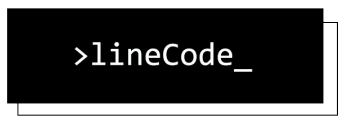
\includegraphics[width=20em]{lclong}
\end{figure}

% Titolo / Nome
\maketitle
\thispagestyle{empty}

% Dati specifici sul doc in forma tabulare
\begin{table}[ht]
	\begin{center}
		\label{tab:Dati sul documento}
		\begin{tabular}{r|l}
			\multicolumn{2}{c}{ \textsc{Dati sul documento} } \\
			\hline
			\textbf{Versione} & \versione{} \\
			\textbf{Uso} & \uso{}  \\
			\textbf{Redattori} & \redattori{} \\
			\textbf{Verificatori} & \verificatori{} \\
			\textbf{Responsabile} & \responsabile{} \\
			\textbf{Destinatari} & lineCode \\
								& prof.\ Vardanega Tullio \\		
								& prof.\ Cardin Riccardo \\
			\ifthenelse{\equal{\uso}{Esterno}}{
								& Sanmarco Informatica
			}{} \\
		\end{tabular}
	\end{center}
\end{table}

\newpage

\renewcommand{\arraystretch}{2} % allarga le righe con dello spazio sotto e sopra
\begin{longtable}[H]{>{\centering\bfseries}m{2cm} >{\centering}m{3.5cm} >{\centering}m{2.5cm} >{\centering}m{3cm} >{\centering\arraybackslash}m{5cm}}
	\rowcolor{lightgray}
	{\textbf{Versione}} & {\textbf{Nominativo}} & {\textbf{Ruolo}} & {\textbf{Data}} & {\textbf{Descrizione}}  \\
	\endfirsthead%
	\rowcolor{lightgray}
	{\textbf{Versione}} & {\textbf{Nominativo}}  & {\textbf{Ruolo}} & {\textbf{Data}} & {\textbf{Descrizione}}  \\
	\endhead%
	\modifiche{}%
\end{longtable}
	\newpage
	\tableofcontents
	\newpage
	\listoffigures
	\listoftables
	\newpage

	%--------------------------------
	%
	% IL CONTENUTO INIZIA DA QUI
	%
	%--------------------------------

	\section{Introduzione}
	\subsection{Scopo del documento}
Il documento ha lo scopo di definire le guidelines del way of working adottato dal team lineCode. Le attività presenti in questo documento sono redatte da processi contenuti nello standard ISO/IEC 12207:1995. Risulta quindi necessario che tutti i membri del gruppo prendano visione di questo documento ai fini di coesione e uniformità all'interno del progetto.

\subsection{Scopo del prodotto}
Il \glock{capitolato} C5 ha come obbiettivo la realizzazione di un applicativo \glock{Real-Time} in grado di guidare delle unità dotate di mobilità autonoma in ambienti specifici, partendo dal presupposto che queste si muovano in ambienti in cui sono presenti altre unità (autonome o meno).

\subsection{Glossario e documenti esterni}
In supporto alla documentazione viene fornito un glossario per chiarire, con una definizione, eventuali termini specifici contenuti in questo documento.
Saranno adottati quindi questi due simboli a pedice:
\begin{itemize}
	\item \textit{D} se indicano un documento specifico;
	\item \textit{G} se incluse nel \dext{glossario}.
\end{itemize}

\subsection{Riferimenti}
	\subsubsection{Riferimenti normativi}
	\begin{itemize}
		\item \textbf{{C5 - PORTACS}}: \url{https://www.math.unipd.it/~tullio/IS-1/2020/Progetto/C5.pdf};
        \item \textbf{Oracle Java Code Conventions}: \url{https://www.oracle.com/technetwork/java/codeconventions-150003.pdf};
        \item \textbf{Angular coding style guide}: \url{https://angular.io/guide/styleguide}.
	\end{itemize}
	\subsubsection{Riferimenti informativi}
	\begin{itemize}
		\item \textbf{ISO/IEC 12207:1995}: \url{https://www.math.unipd.it/~tullio/IS-1/2009/Approfondimenti/ISO_12207-1995.pdf};
		\item \textbf{Gitflow}: \url{http://nvie.com/posts/a-successful-git-branching-model/};
		\item \textbf{Documentazione Zapier}: \url{https://zapier.com/help};
		\item \textbf{Documentazione act}: \url{https://github.com/nektos/act/blob/master/README.md};
		\item \textbf{Studio di Fattibilità}: \dext{Studio di Fattibilità v1.0.0};
		\item \textbf{Piano di Qualifica}: \dext{Piano di Qualifica v2.0.0};
		\item \textbf{Piano di Progetto}: \dext{Piano di Progetto v2.0.0}.
	\end{itemize}
	\newpage

	\section{Tecnologie utilizzate}
	\begin{table} [h!]
	\rowcolors{2}{gray!25}{gray!6}
	\begin{center}
		\begin{tabular} { m{5cm} m{12cm} }
			\rowcolor{lightgray}
			\textbf{Tecnologia} & \textbf{Utilizzo} \\
			\glock{Angular} & Implementa l'interfaccia grafica del programma \\
			\glock{AsciiDoc} & Utilizzato per sviluppare il documento dedicato ai test \\
			\glock{Chai} & Utilizzato per gli unit test dell'unità \\
			\glock{Checkstyle} & Controlla il codice \glock{Java} del server \\
			\glock{Docker} & Le componenti del software sono contenuti in vari container di questa tecnologia \\
			\glock{ESLint} & Controlla il codice \glock{JavaScript} dell'interfaccia grafica \\
			\glock{GitHub} & Tutto il progetto sfrutta questo servizio ed i suoi strumenti \\
			\glock{Jasmine} & Utilizzato per gli unit test test dell'interfaccia grafica\\
			\glock{Java} & Tutta la parte del server è sviluppata in \glock{Java} \\
			\glock{JSON} & Il formato è stato utilizzato nelle comunicazioni da e per il server \\
			\glock{JUnit} & Tutti i test di unità del server utilizzano questo \glock{framework} \\
			\glock{\LaTeX} & Quasi tutti i documenti sono stati prodotti utilizzando questo linguaggio \\
			\glock{Maven} & È stato utilizzato nello sviluppo del server \\
			\glock{Mocha} & Utilizzato per gli unit test dell'unità \\
			\glock{NPM} & Gestisce il codice della UI e dell'unità \\
			\glock{Redis} & Utilizzato per la persistenza dei dati del server \\
			\glock{SonarCloud} & Utilizzato nella \glock{Continuous Integration} \\
			\glock{Typescript} & Codice delle unità e dell'interfaccia \\
		\end{tabular}
		\caption{Lista delle tecnologie utilizzate}
	\end{center}
\end{table}

	\newpage

	\section{Requisiti di sistema}
	\subsection{Requisiti minimi di sistema}

	\subsubsection{Requisiti hardware}
	I requisiti hardware del progetto corrispondono a quelli di Docker:
	\begin{itemize}
		\item processore a 64 bit con Second Level Address Translation (SLAT);
		\item RAM di sistema da 4 GB;
		\item il supporto per la virtualizzazione hardware a livello di BIOS deve essere abilitato nelle impostazioni del BIOS.
	\end{itemize}  
	
	\subsubsection{Requisiti software}
	Il software è stato testato in tutti e tre gli ambienti più utilizzati:
	\begin{itemize}
		\item Linux Ubuntu 18.04 LTS o successiva; 
		\item macOS 10.14 o successiva;
		\item Windows 10 a 64bit build 19041 o successiva.
	\end{itemize}  
	
\subsection{Installazione}

	\subsubsection{Ambiente di lavoro}

	\subsubsection{Librerie}

	\newpage

	\section{Test}
	
La classificazione dei test è riportata alla sezione Verifica delle \dext{Norme di progetto v2.0.0}. \\

\subsection{Tipologie di test}
I test saranno di quattro tipologie:
\begin{itemize}
	\item \textbf{Test di Sistema [TS] };
	\item \textbf{Test di Accettazione [TA]};
	\item \textbf{Test di Integrazione [TI]};
	\item \textbf{Test di Unità [TU]}.\\
\end{itemize}

\subsubsection{Test di sistema}

	\newcommand*{\thead}[1]{\multicolumn{1}{c}{\bfseries #1}}	
	\rowcolors{2}{gray!6}{gray!25}
	\setlength{\tabcolsep}{10pt}
	\begin{longtable}[h!] { c  m{12cm} c}
		\caption{Test di Sistema} \\
		\rowcolor{lightgray}
		\thead{Test}  & \thead{Descrizione} & \thead{Esito} \\ \endhead%
	
		TSMF1   & La mappa deve essere disponibile per l'utente generico in sola lettura	& NI \\
		
		TSMF1.1 & L'utente generico deve poter visualizzare la legenda dei simboli utilizzati all'interno della mappa & NI \\
		
		TSFM1.2 & La mappa deve aggiornarsi periodicamente, mostrando le informazioni sul movimento delle unità che fanno parte del sistema & NI\\
		
		TSDM1.3 & La mappa deve mostrare le informazioni sui pedoni che comunicano con il sistema & NI \\
		
		TSFM1.4 & La mappa deve essere visualizzabile per ogni tipo di utente & NI\\
		
		
		TSFM2   & L'utente registrato deve poter effettuare il login. All'utente viene chiesto di:
				\begin{itemize}
					\item accedere all'area login;
					\item inserire il nome utente;
					\item inserire la password.
				\end{itemize}
								& NI \\
								
		TSFM2.1 & L'utente deve visualizzare un messaggio di errore nel caso in cui:
					\begin{itemize}
						\item viene fornito un nome utente non esistente;
						\item viene fornita una password errata.
					\end{itemize}
									& NI \\		
		TSFM3   & L'utente autenticato deve poter effettuare il logout dal sistema. L'utente può verificare che la disconnessione sia avvenuta con successo & NI \\
		
		TSFM4   & La guida utente deve essere visualizzabile dai soli utenti registrati & NI \\
									
		TSFM4.1 & La guida utente deve contenere tutte le istruzioni che un utente può svolgere all'interno del sistema & NI \\
		
		TSFM5   & L'utente autenticato deve poter visualizzare la lista delle unità attive con il proprio ID & NI \\
		
		TSFM5.1 & Ogni elemento della lista di unità fornisce un ambiente grafico per la gestione delle proprietà dell'unità selezionata & NI \\
		
		TSFO5.2 & L'utente autenticato, dentro l'ambiente grafico, deve visualizzare l'ID dell'unità selezionata & NI \\
		
		TSFM5.3 & L'utente autenticato deve poter visualizzare le seguenti informazioni dell'unità:
					\begin{itemize}
						\item le coordinate della posizione attuale all'interno della mappa;
						\item lo stato in cui si trova;
						\item la velocità attuale;
						\item la direzione del prossimo passo suggerita dal sistema;
						\item la coda degli ordini assegnati.
					\end{itemize}	
									&NI\\
				
		TSFM5.4  & L'utente autenticato deve poter impartire i seguenti comandi all'unità:
					\begin{itemize}
						\item \underline{Start};
						\item \underline{Stop};
						\item \underline{Go Back};
						\item \underline{Shutdown}.
					\end{itemize}
									& NI \\
									
		TSFM5.5  & L'utente autenticato deve poter aggiungere un nuovo ordine alla coda degli ordini assegnati all'unità & NI\\
		
		TSFM5.6  & L'utente autenticato deve poter eliminare un ordine alla coda degli ordini assegnati all'unità & NI\\
		
		TSFM6 & L'amministratore deve poter visualizzare la lista degli utenti registrati, con le seguenti informazioni:
					\begin{itemize}
						\item nome utente;
						\item password.	
					\end{itemize}
									& NI \\
		TSFM6.1 & L'amministratore deve poter creare un nuovo utente. Il sistema richiede in input le seguenti credenziali:
					\begin{itemize}
						\item nome utente;
						\item password;
						\item status.
					\end{itemize}
										& NI \\
										
		TSFM6.2  & L'amministratore deve poter modificare un utente registrati. Il sistema richiede in input le seguenti credenziali:
					\begin{itemize}
						\item nome utente;
						\item password.
					\end{itemize}
											& NI \\
		TSFM6.3 & L'amministratore deve poter eliminare un utenti registrato & NI \\
		
		TSFM6.4 & L'amministratore deve visualizzare un messaggio di errore nel caso in cui:
						\begin{itemize}
						\item il nome utente inserito sia già esistente; 
						\item la password non è formattata correttamente.
					\end{itemize}
										& NI \\
		TSFM7   & L'amministratore per poter modificare la mappa, deve poter inserire un file da validare & NI\\
		
		TSFM7.1 & L'amministratore deve visualizzare un messaggio di errore nel caso in cui il file non sia formattato correttamente & NI \\
		
		TSFM8   & L'amministratore deve poter visualizzare la lista delle unità registrate, con il proprio ID & NI\\
		
		TSFM8.1 & L'amministratore deve poter aggiungere una nuova unità alla liste delle unità registrate. Il sistema richiede in input l'ID & NI\\	
		
		TSFM8.2 & 	L'amministratore deve poter modificare la lista delle unità registrate. Il sistema richiede in input il rispettivo ID & NI\\
		
		TSFM8.3 & L'amministratore deve poter eliminare una unità dalla lista & NI\\
		
		TSFM8.4  & L'amministratore deve visualizzare un messaggio d'errore nel caso venga fornito un ID già esistente & NI \\
		
		TSFM9   & L'unità, dotata di sensoristica, deve comunicare al sistema la posizione relativa degli ostacoli che riescono a rilevare & NI \\
		
		TSFM10 & Il sistema deve ricevere le coordinate dall'unità sulla sua posizione attuale & NI \\
		
		TSFM11 & L'unità deve avere un percorso fornito dal sistema per raggiungere il prossimo \glock{POI} & NI \\
		
		TSFM12 & L'unità deve avere una lista di \glock{POI} da raggiungere & NI \\
		
		TSFM13  & L'utente autenticato può modificare la lista deglli ordini solo quando l'unità si trova in una base di ricarica & NI \\
		
		TSFM14  & L'unità, con coda degli ordini vuota, deve ritornare nella base di ricarica & NI \\
		
		TSFM15  & L'unità non può superare un certo limite di velocità & NI \\
		
		TSFM16 & L'unità può assumere uno dei seguenti stati:
				\begin{itemize}
					\item \underline{Going to X};
					\item \underline{Stop};
					\item \underline{Base};
					\item \underline{Error Y}.
				\end{itemize}		
										& NI \\
										
		TSFM17  & Il sistema dispone di un algoritmo che deve:
				\begin{itemize}
					\item calcolare il percorso che l'unità deve percorrere per raggiungere il \glock{POI};
					\item evitare la collisione con altre unità;
					\item evitare la collisione con gli ostacoli.
				\end{itemize}		
										& NI \\
		
		TSFO18  & Il percorso restituito dall'algoritmo, è un percorso ottimo & NI\\
		
		TSFD19 & Il sistema riceve dal pedone le informazioni sulla sua posizione & NI\\

		TSFD20  & Il sistema riconosce il pedone come un ostacolo & NI \\
		\hline
		
		TSMC1   & Deve essere fornito un documento con i casi d'uso in formato UML & NI \\
		
		TSMC2   & Deve essere consegnato uno schema relativo al design della base di dati & NI \\
		
		TSMC3  &Deve essere consegnata la documentazione delle \glock{API} realizzate & NI\\
		
		TSMC4   & Deve essere consegnata una lista di bug risolti durante lo sviluppo & NI\\
		
		TSMC5   & Il codice sorgente del prodotto dovrà essere versionato con \glock{GitHub} & NI\\
		
		TSMC6   & Ogni entità sviluppata facente parte del sistema dovrà essere contenuta in un container \glock{Docker} & NI \\
		
		TSMC7   & Deve essere fornito un \glock{Dockerfile} contenente:
						\begin{itemize}
							\item il motore di calcolo;
							\item il visualizzatore \glock{Real-Time}.
						\end{itemize} 
											& NI \\
											
		TSMC7.1 & Deve essere fornito un \glock{Dockerfile} per la singola unità & NI \\
		
		TSD7.2 &  Deve essere fornito un \glock{Dockerfile} per il singolo pedone & NI \\
		
		TSMC8  & L'astrazione della mappatura dell'ambiente dovrà rispettare una struttura a griglia con divisione in celle & NI \\
		
		\hline
		
		TSMQ1 & Il prodotto va rilasciato con la licenza \glock{open-source} più aperta possibile in base alle librerie utilizzate & NI \\
		
		TSMQ2 & Il prodotto deve essere conforme con quanto dichiarato nel documento \dext{ Piano di Qualifica v2.0.0} & NI \\
		
		TSMQ3  & Devono essere realizzati test di unità e di integrazione per vericare le singole componenti del prodotto & NI \\
		
		\hline
		
		TSMP1  &  Il tempo di aggiornamento della mappatura rispetto alla posizione delle unità nell'ambiente deve essere $\geq$ 5 secondi & NI \\
	
		TSDP1.1  & Il tempo di aggiornamento della mappatura rispetto alla posizione delle unità nell'ambiente deve essere $\geq$ 2.5 secondi & NI \\
		
		TSOP1.2  &  Il tempo di aggiornamento della mappatura rispetto alla posizione delle unità nell'ambiente deve essere $\geq$ 1 secondi & NI \\
										
		TSMP2	& Il servizio non deve mai essere interrotto secondo una logica di \glock{zero downtime}	& NI \\\\									
\end{longtable}

\subsubsection{Test di accettazione}
I test di Accettazione hanno lo scopo di dimostrare che il prodotto sviluppato soddisfi i requisiti presenti nel capitolato e concordati con il proponente e, con quest'ultimo, eseguito durante il collaudo finale del prodotto. 

\subsubsection{Test di integrazione}
Le specifiche di questi test verranno scritte successivamente rispettando il \glock{Modello a V}.
\subsubsection{Test di Unità}
Le specifiche di questi test verranno scritte successivamente rispettando il \glock{Modello a V}.





	\newpage

	\section{Architettura}
	\subsection{Descrizione generale}
	Durante la fase di progettazione la struttura del prodotto è stata modellata in quattro componenti distinte:
	\begin{itemize}
		\item \textbf{server}: motore di calcolo che coordina le unità e genera le informazioni per la UI; viene modellato seguendo la \textit{layered architecture};
		\item \textbf{interfaccia grafica}: mostra la mappa e permette di gestire le unità e gli utenti; viene modellata seguendo il \textit{MVVM};
		\item \textbf{unità}: si occupa di simulare il comportamento di un'unità all'interno dell'ambiente; viene modellata seguendo la \textit{hexagonal architecture};
		\item \textbf{sensori}: si occupa di simulare il comportamento dei sensori delle unità all'interno dell'ambiente; non viene modellato secondo una architettura specifica poiché triviale.
	\end{itemize}
	La UI e l'unità comunicano con il server tramite l'uso di \glock{WebSocket} e lo scambio di messaggi \glock{JSON}. Il server, quindi, conoscendo la posizione di tutte le unità e ostacoli, genera il percorso migliore, lo comunica alle unità richiedenti e aggiorna la mappa informando l'interfaccia grafica.\\

\subsection{Architettura del server}
	Il pattern architetturale applicato alla componente server è la \textit{Layered Architecture}. \\
	Si è scelto tale pattern in quanto la componente server risulta troppo complessa per essere destrutturata dovendo gestire i servizi di: anagrafica unità, anagrafica utente, gestione mappa, calcolo percorsi unità e gestione delle interfacce grafiche.\\
	Di seguito viene illustrato il diagramma dei package. Si noti che le dipendenze procedono in un'unica direzione senza creare cicli. Si noti, inoltre, che il sistema dipende dalla classe \textbf{Position} in ogni suo punto in quanto, trattando problematiche legate al movimento di un'unità in una griglia, avere un tipo di dato che rappresenti due coordinate cartesiane risulta particolarmente utile.

	\begin{figure}[H]
		\centering
		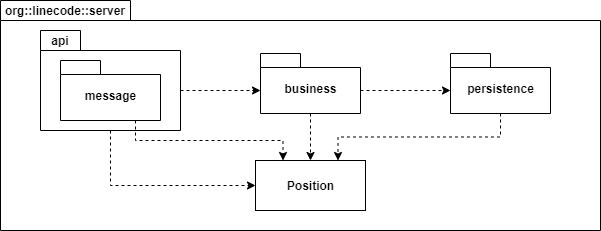
\includegraphics[width=12cm]{img/server_package.png}
		\caption{Server - Diagramma dei package}
	\end{figure}
	
	\begin{figure}[H]
		\centering
		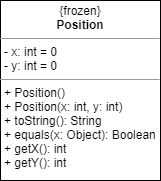
\includegraphics[width=4cm]{img/class_position.png}
		\caption{Server - Classe Position}
	\end{figure}

	\subsubsection{Messaggi}
		È stato stabilito un formato standard di messaggi da e per UI e unità. Tali messaggi sono rappresentati come classi \glock{Java} e verranno scambiati con le altre componenti del prodotto in seguito alla loro serializzazione e deserializzazione in formato \glock{JSON}.\\
		Tutte le classi (vedi figure 3 e 4) estendono la classe astratta Message.
	
		\begin{landscape}
			\begin{figure}[]
				\centering
				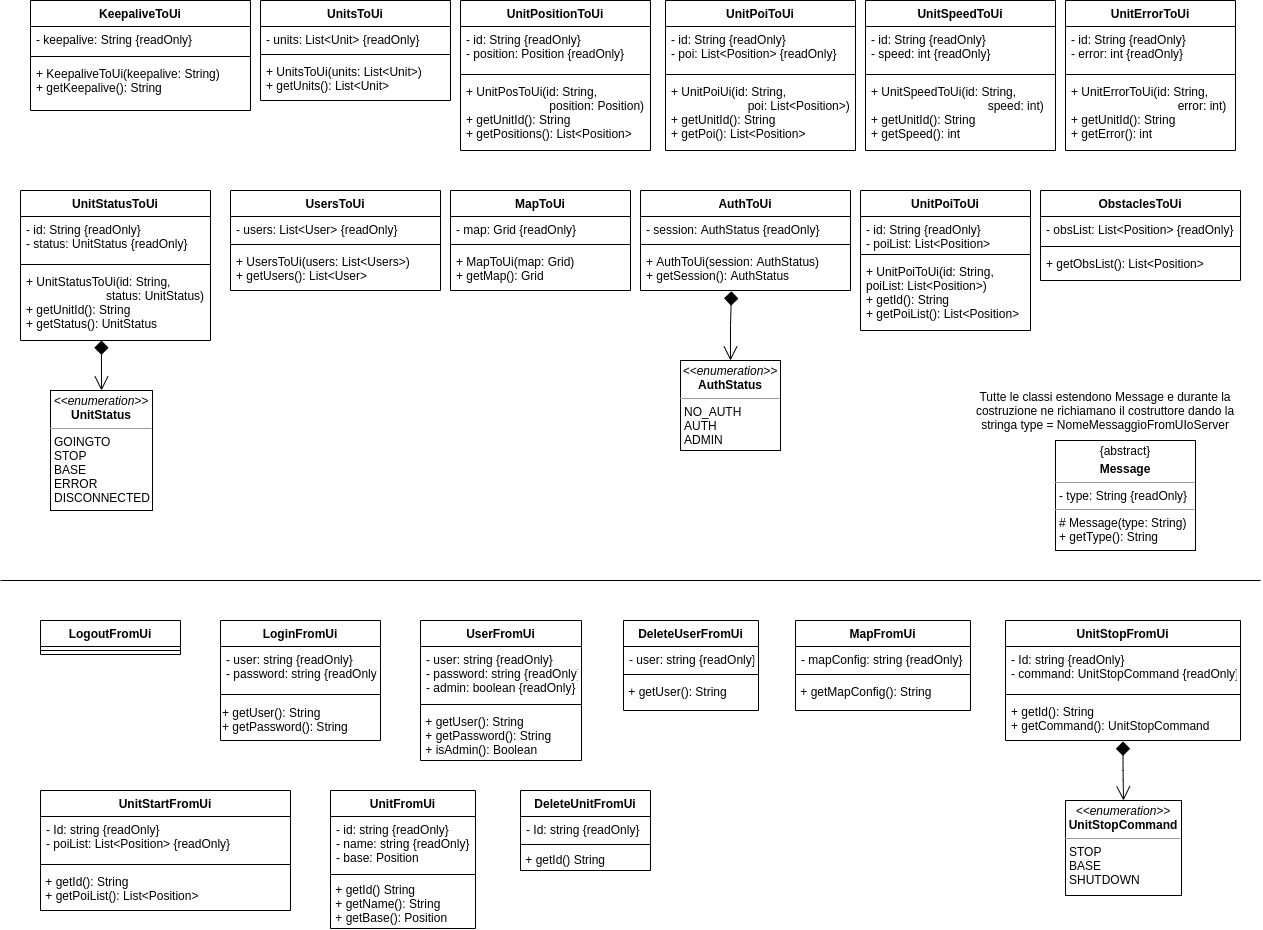
\includegraphics[width=23cm]{img/server_from_to_ui.png}
				\caption{Server - Messaggi da e per l'interfaccia}
			\end{figure}
		\end{landscape}
		\begin{landscape}

			\begin{figure}[H]
				\centering
				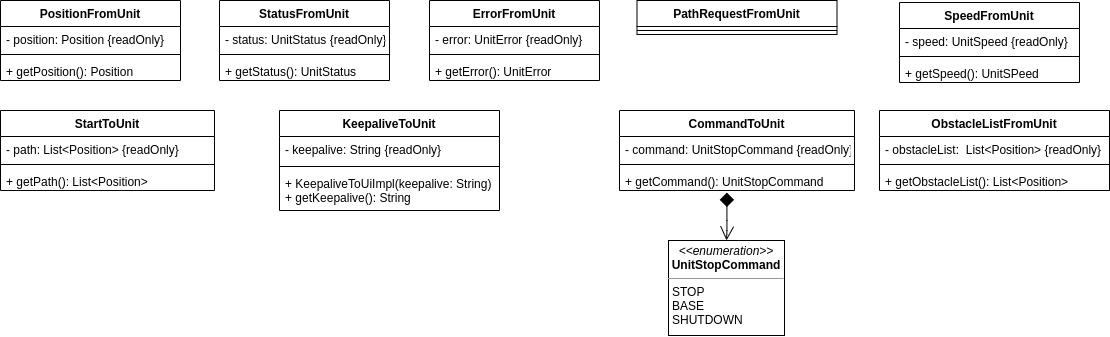
\includegraphics[width=22cm]{img/server_from_to_unit.png}
				\caption{Server - Messaggi da e per l'unità}
			\end{figure}
		\end{landscape}

	\subsubsection{API layer}
		Qui troviamo i metodi che permettono la gestione della connessione alle altre componenti del sistema, e quindi anche l'invio e la ricezione di messaggi mediante opportune serializzazioni e deserializzazioni. Il tutto viene gestito dallo standard JRS 356 per i \glock{WebSocket} e da \glock{Jackson} per la (de)serializzazione.

	\subsubsection{Business layer}
		Qui troviamo la logica per l'elaborazione dei dati. Le informazioni scendono in questo layer tramite chiamata a funzione da parte dell'API layer su opportune interfacce. I prodotti dell'elaborazione vengono riportati nel layer superiore tramite oggetto ritornato dai metodi oppure, quando l'oggetto chiamante non è lo stesso che deve ricevere quanto ritornato, tramite l'emissione di opportuni segnali che verranno intercettati dal layer sovrastante secondo una logica \glock{signal/slot} simile alla libreria grafica \glock{Qt} fornita dalla libreria \glock{Sig4j}. Lo slot viene consegnato tramite chiamata a funzione dall'API layer alla costruzione dell'istanza Endpoint in modo che possa avvenire la connessione fra segnale e slot. In tal modo viene messo in atto un sistema di scambio dei messaggi "dal basso verso l'alto" mantenendo la direzione delle dipendenze in senso contrario.

	\subsubsection{Persistence layer}
		Qui troviamo le classi che permettono al Business layer di relazionarsi con il database indipendentemente dall'implementazione dello stesso grazie all'uso di opportune interfacce.

		\begin{landscape}
			\begin{figure}[h!]
				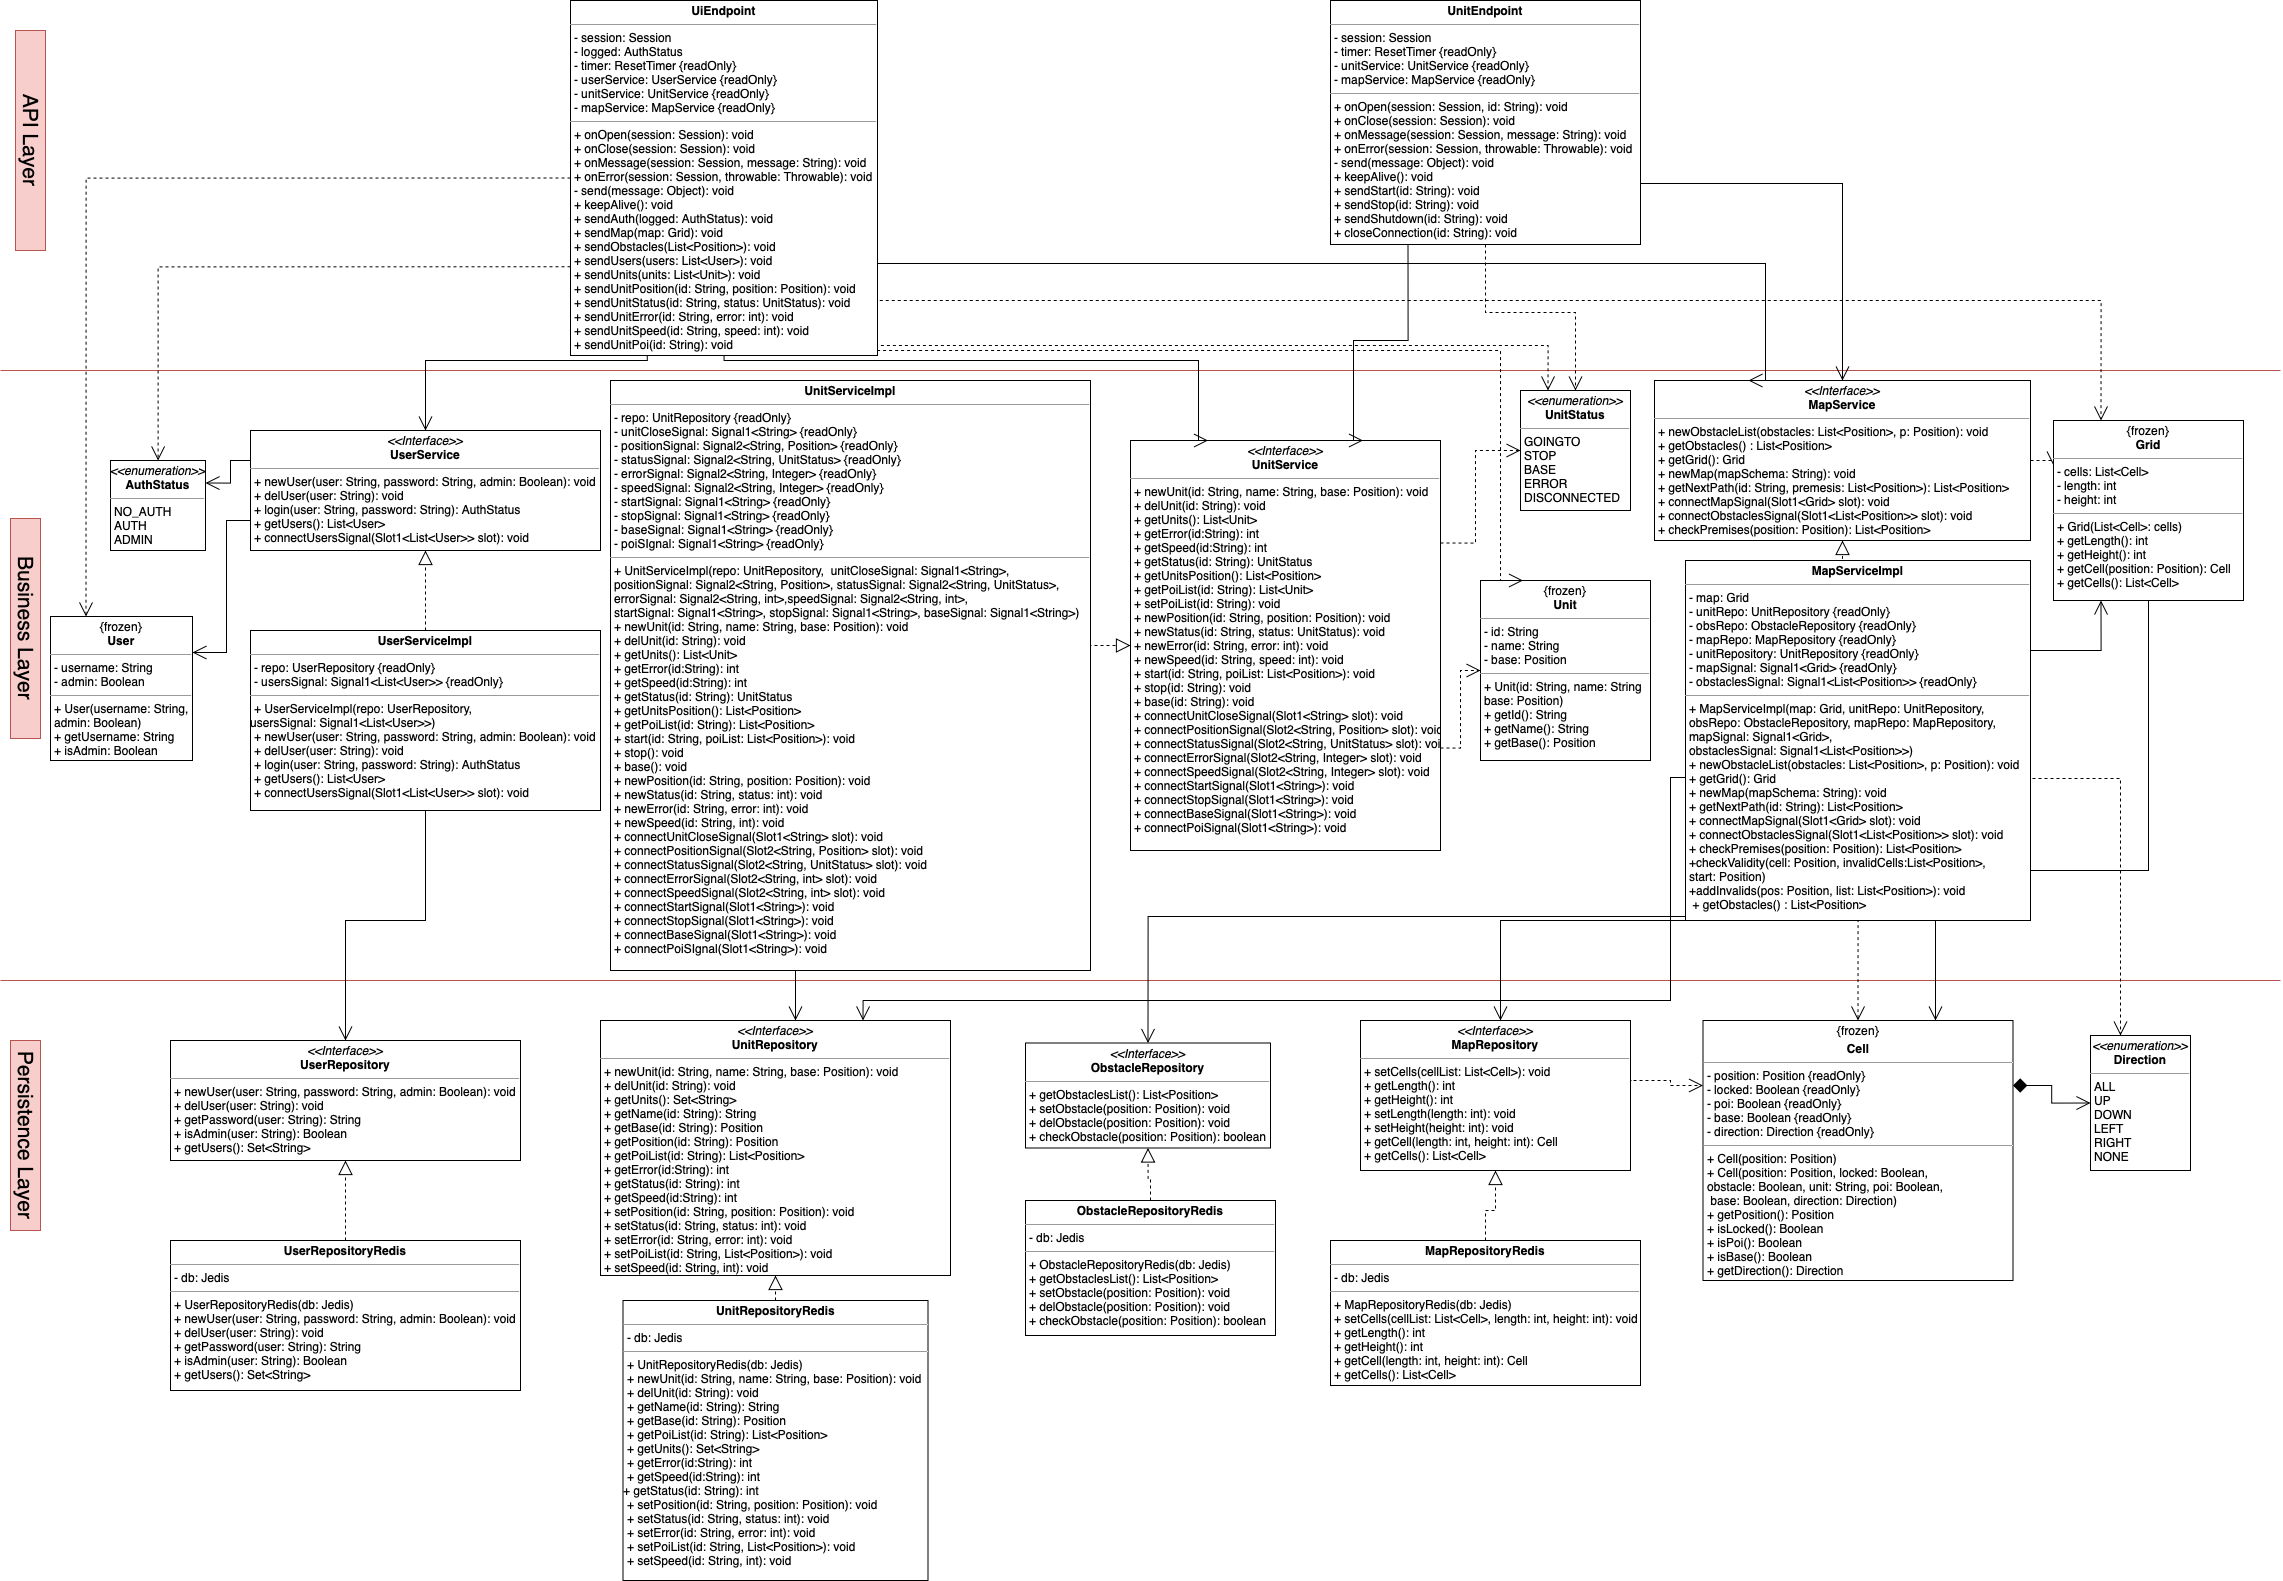
\includegraphics[width=26cm]{img/server_classi.png}
				\caption{Server - Diagramma delle classi}
			\end{figure}
		\end{landscape}
	
	\subsubsection{Database layer}
		Per garantire le migliori performance al sistema e vista la quantità non eccessiva di dati, si è scelto \glock{Redis} come database essendo esso \glock{in-memory}. Non esistono diagrammi standard per rappresentarne la struttura dunque verranno elencate le strutture dati nella tabella seguente:
		
		\begin{table} [h!]
			\rowcolors{2}{gray!25}{gray!6}
			\begin{center}
				\begin{tabular} { m{6cm} m{4cm} m{2cm} m{4cm}}
					\rowcolor{lightgray}
					\textbf{Descrizione} & \textbf{Key} & \textbf{Tipo} & \textbf{Valori / Campi Dati}\\
					id delle unità & unit & SET & \\
					dati e anagrafica delle unità & unit:[id\_unit] & HASH & 
						\begin{itemize}
							\item name
							\item base\_x
							\item base\_y
							\item position\_x
							\item position\_y
							\item status
							\item error
							\item speed
						\end{itemize}\\
					coordinate \glock{POI} da raggiungere per una specifica unità & poi:[id\_unit] & LIST & [coord\_x]:[coord\_y]\\
					username degli user & user & SET & \\
					anagrafica degli user & user:[username] & HASH & 
						\begin{itemize}
							\item password
							\item admin
						\end{itemize}\\
					lunghezza tabella (asse x) & length & STRING & \\
					altezza tabella (asse y) & height & STRING & \\
					dati delle celle della mappa & cell:[coord\_x]:[coord\_y] & HASH & 
						\begin{itemize}
							\item locked
							\item base
							\item direction
							\item poi
						\end{itemize}\\
					id degli ostacoli (intero incrementale) con posizione & obs:[id\_obs] & LIST & [coord\_x]:[coord\_y]\\
				\end{tabular}
				\caption{Struttura del database \glock{Redis}}
			\end{center}
		\end{table}
	
		\newpage
	
		\begin{landscape}
			\subsubsection{Diagrammi di sequenza}
			Il seguente diagramma rappresenta il caso in cui l'interfaccia grafica invii al server una lista di \glock{POI}, che l'unità deve raggiungere.\\
			\begin{figure}[H]
				\centering
				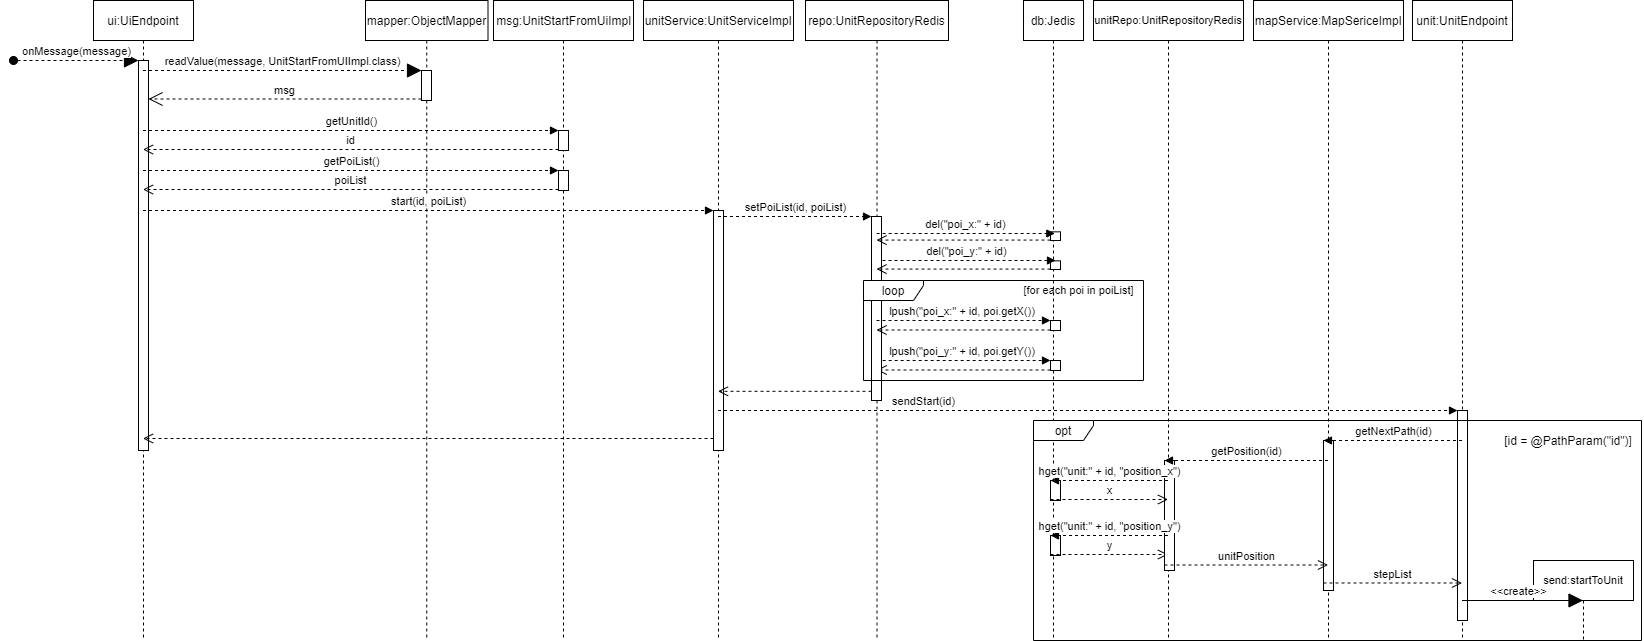
\includegraphics[width=25.7cm]{img/server_seq1.png}
				\caption{Server - UI invia una lista di \glock{POI} che l'unità deve raggiungere}
			\end{figure}
		\end{landscape}
		
		\newpage
		
		\begin{landscape}
			Il seguente diagramma rappresenta il caso in cui un utente esegua il login dall'interfaccia grafica.
			\begin{figure}[H]
				\centering
				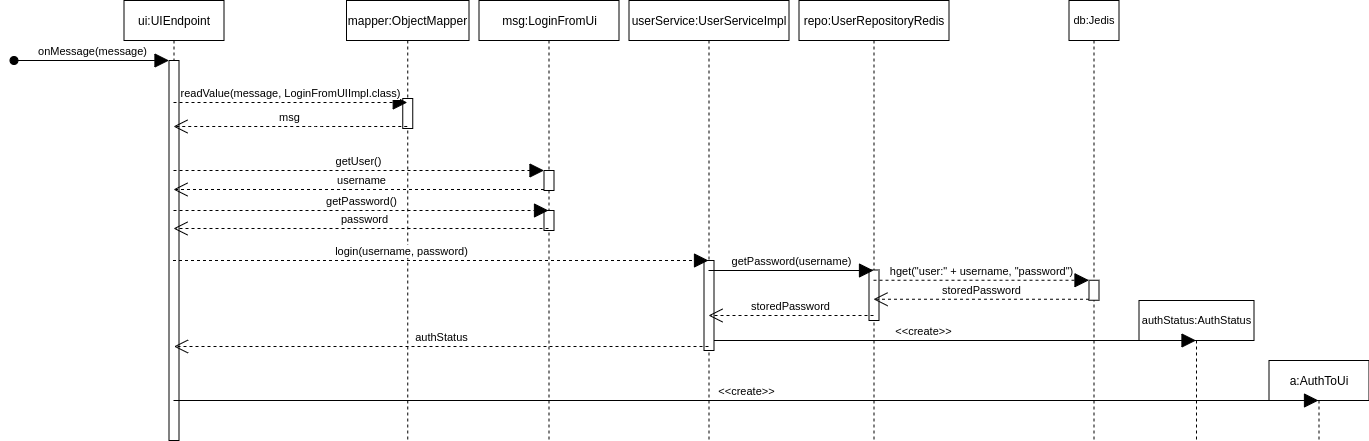
\includegraphics[width=25.7cm]{img/server_seq2.png}
				\caption{Server - Richiesta di login da parte della UI}
			\end{figure}
		\end{landscape}

		\newpage

		\begin{landscape}
			Il seguente diagramma rappresenta il caso in cui un utente elimini un'unità registrata.
			\begin{figure}[H]
				\centering
				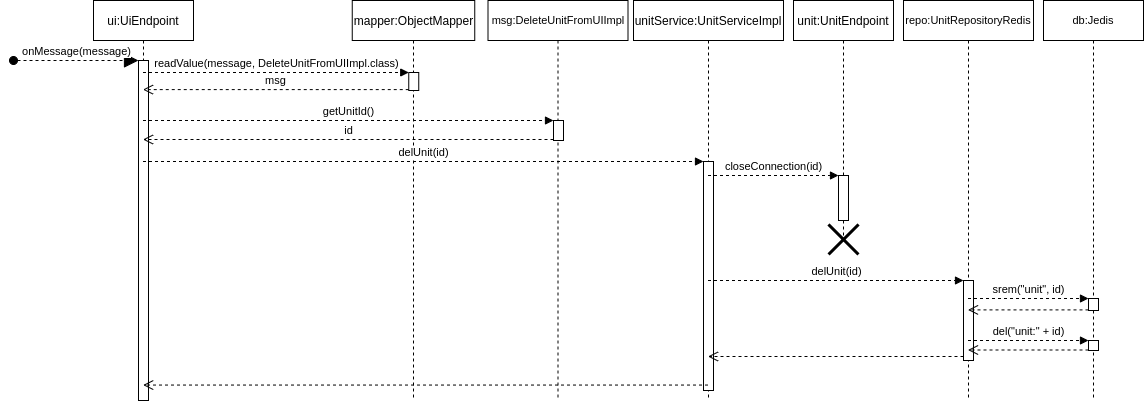
\includegraphics[width=25.7cm]{img/server_seq3.png}
				\caption{Server - UI richiede eliminazione unità}
			\end{figure}
		\end{landscape}
	
\subsection{Architettura dell'interfaccia}
	L'interfaccia grafica è realizzata tramite il framework \glock{Angular}, per questo motivo, il design architetturale utilizzato è il \textit{Model View ViewModel} (\textit{MVVM}) che è intrinseco nel framework stesso. \\
	\newline
	La comunicazione con il server avviene tramite \glock{WebSocket} ed è dunque asincrona. 
	Inoltre, per garantire l'estensibilità del codice, il servizio \textit{WebSocketService} implementa l'interfaccia \textit{ServerService} che mette a disposizione i metodi per interfacciarsi con il server. In questo modo un cambio di tecnologia, ad esempio passando a richieste \glock{HTTP}, non comporterebbe uno stravolgimento dell'architettura. \\
	Per lo stesso motivo sono previste delle interfacce per rappresentare i vari tipi di messaggi che vengono ricevuti dal server, successivamente implementate per specificarne le caratteristiche. \\
	Ogni componente che fa parte del \textit{ViewModel} rappresenta una funzionalità principale che l'interfaccia mette a disposizione all'utente.\\
	\newline
	L'aggiornamento dei dati tra gli \glock{Angular Components} ed il \glock{WebSocket} avviene tramite l'uso dei \glock{Subject} (uno per tipo) al'interno di quest'ultimo; indirizzando tali dati  ai componenti che prevedono appositi campi dati per ricevere le informazioni.
	Inoltre il \textit{WebSocketService} contiene dei campi dati per ritenere gli ultimi dati ricevuti dal server per ogni tipo di dato, in modo tale che alla generazione di un nuovo componente, \glock{Angular} questo abbia a disposizione i dati di cui necessita. \\
	\newline
	Di seguito due diagrammi delle classi: il primo per descrivere il legame tra \textit{Model} e \textit{Viewmodel}, con la struttura dei vari \glock{Angular} Components, mentre la parte di \textit{View}; che comprende i templates degli \glock{Angular} Components, non viene qui rappresentata perché la struttura del codice è \glock{HTML}.
	Il secondo, invece, rappresenta i messaggi che vengono inviati e ricevuti dal server.
	\newpage
	
	\begin{landscape}
		\begin{figure}[h!]
			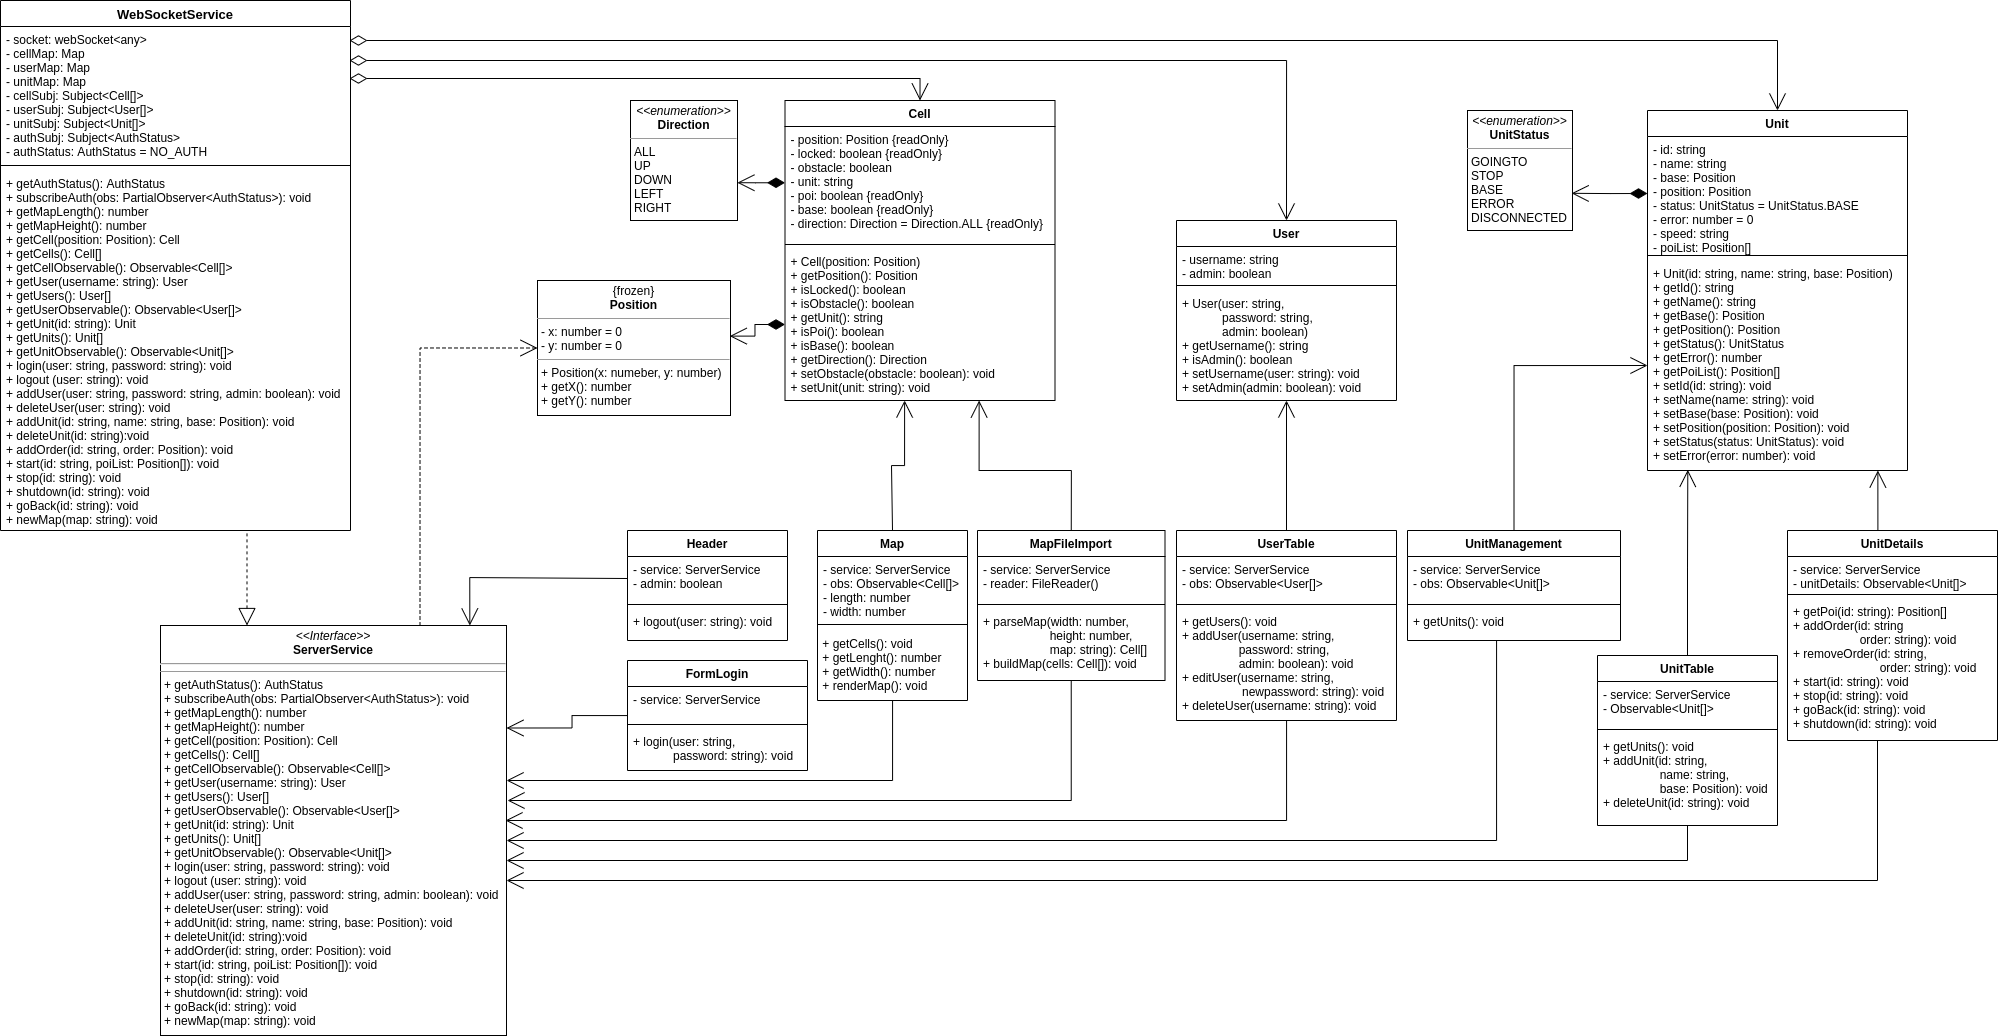
\includegraphics[width=24cm]{img/ui_component.png}
			\caption{Architettura dell'interfaccia - Model-View Model}
		\end{figure}
	\end{landscape}
	\newpage
	
	\begin{landscape}
		\begin{figure}[h!]
			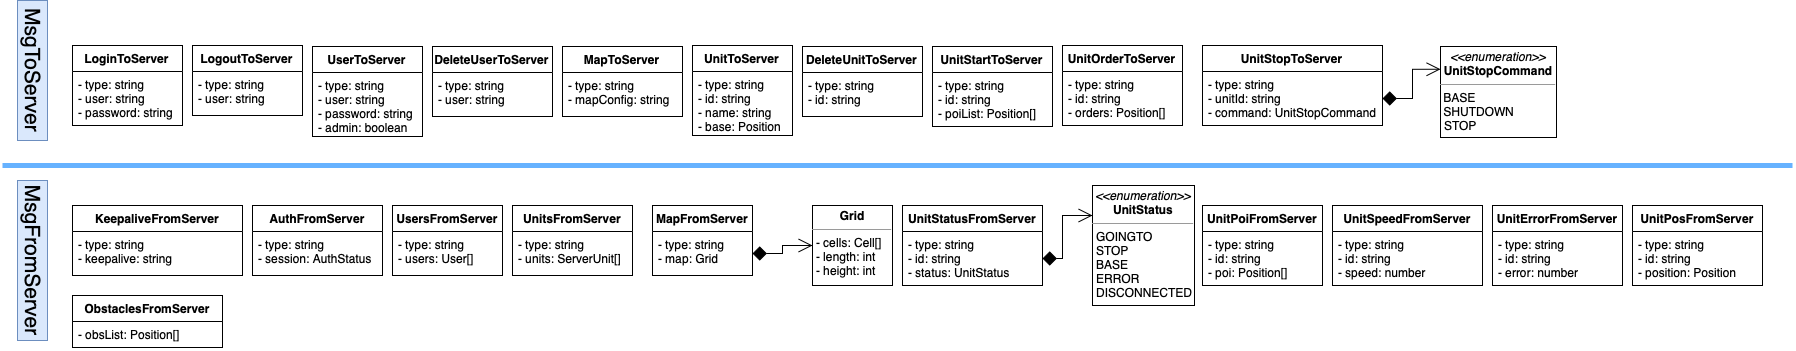
\includegraphics[width=24cm]{img/ui_messaggi.png}
			\caption{Architettura dell'interfaccia - Messaggi}
		\end{figure}
	\end{landscape}

\subsection{Architettura delle unità}
	La componente relativa all'unità viene sviluppata utilizzando il run-time \glock{Node.JS} e i \glock{WebSocket} per la comunicazione con le componenti del server e dei sensori, mentre per lo strato di persistenza si è deciso di fare utilizzo del database \glock{MongoDB}.
	La scelta architetturale per questa componente è ricaduta sulla \textit{Hexagonal Architecture}.
	I motivi riconducibili alla suddetta scelta sono da riscontrarsi nella natura semplicistica del servizio che la componente mette a disposizione. Le logiche di business si occupano unicamente di controllare che i dati ricevuti (già validati nel formato) vengano esaminati e processati per poi essere salvati sul persistence layer.
	Il punto fondamentale è che, oltre ai controller, anche la classe \textit{UnitEngine} si occupa di scrivere e leggere dati dallo strato di persistenza, in modo da emulare l'evolvere degli stati mano a mano che l'unità avanza lungo il percorso e/o incontra ostacoli.
	È inoltre prevista, similmente a quanto accade per la parte relativa alla UI, una gerarchia di interfacce e classi che si occupano di modellare tutti i possibili messaggi che l'unità può voler scambiare con le altre componenti, in modo da controllare in maniera più pulita il passaggio di informazioni.
	Per quanto concerne i sensori, invece, essi non sono dotati di una reale architettura, data la trivialità del loro scopo e del modo in cui il componente opera per raggiungerlo.
	
	\begin{figure}[H]
		\centering
		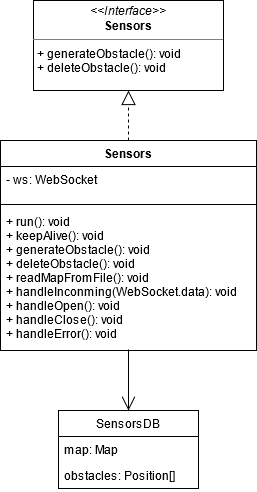
\includegraphics[width=6cm]{img/unit_sensori.png}
		\caption{Unità - Sensori}
	\end{figure}
	
	Di seguito si illustrano i diagrammi delle classi dell'architettura dell'unità, e dei messaggi usati per interfacciarsi con il server.
	
	\begin{landscape}
		\begin{figure}[h!]
			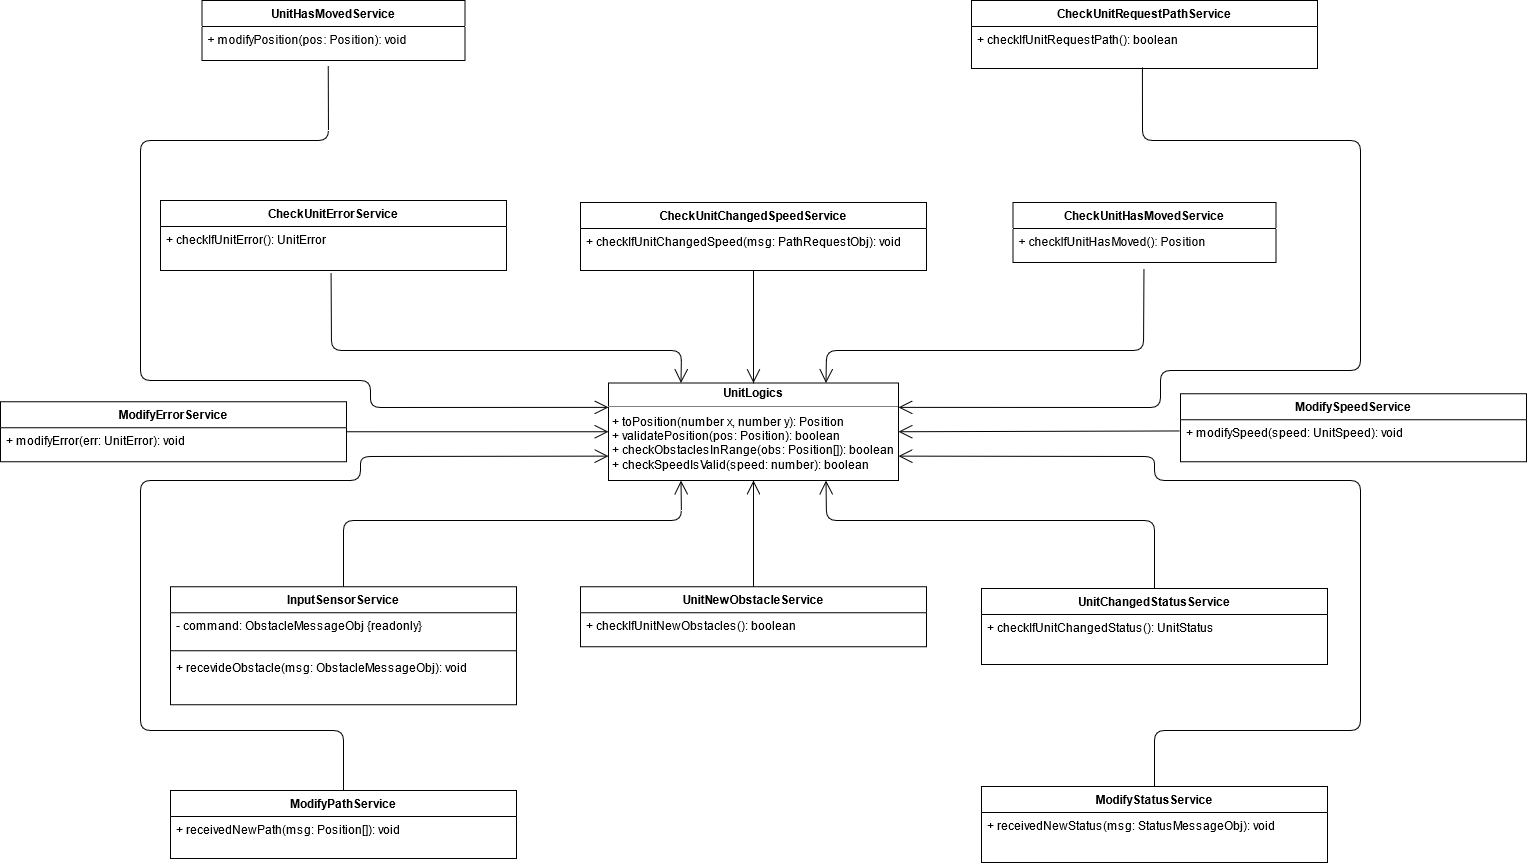
\includegraphics[width=25.5cm]{img/unit_architettura1.png}
			\caption{Unità - Diagramma delle classi}
		\end{figure}
	\end{landscape}
	
	\begin{landscape}
		\begin{figure}[h!]
			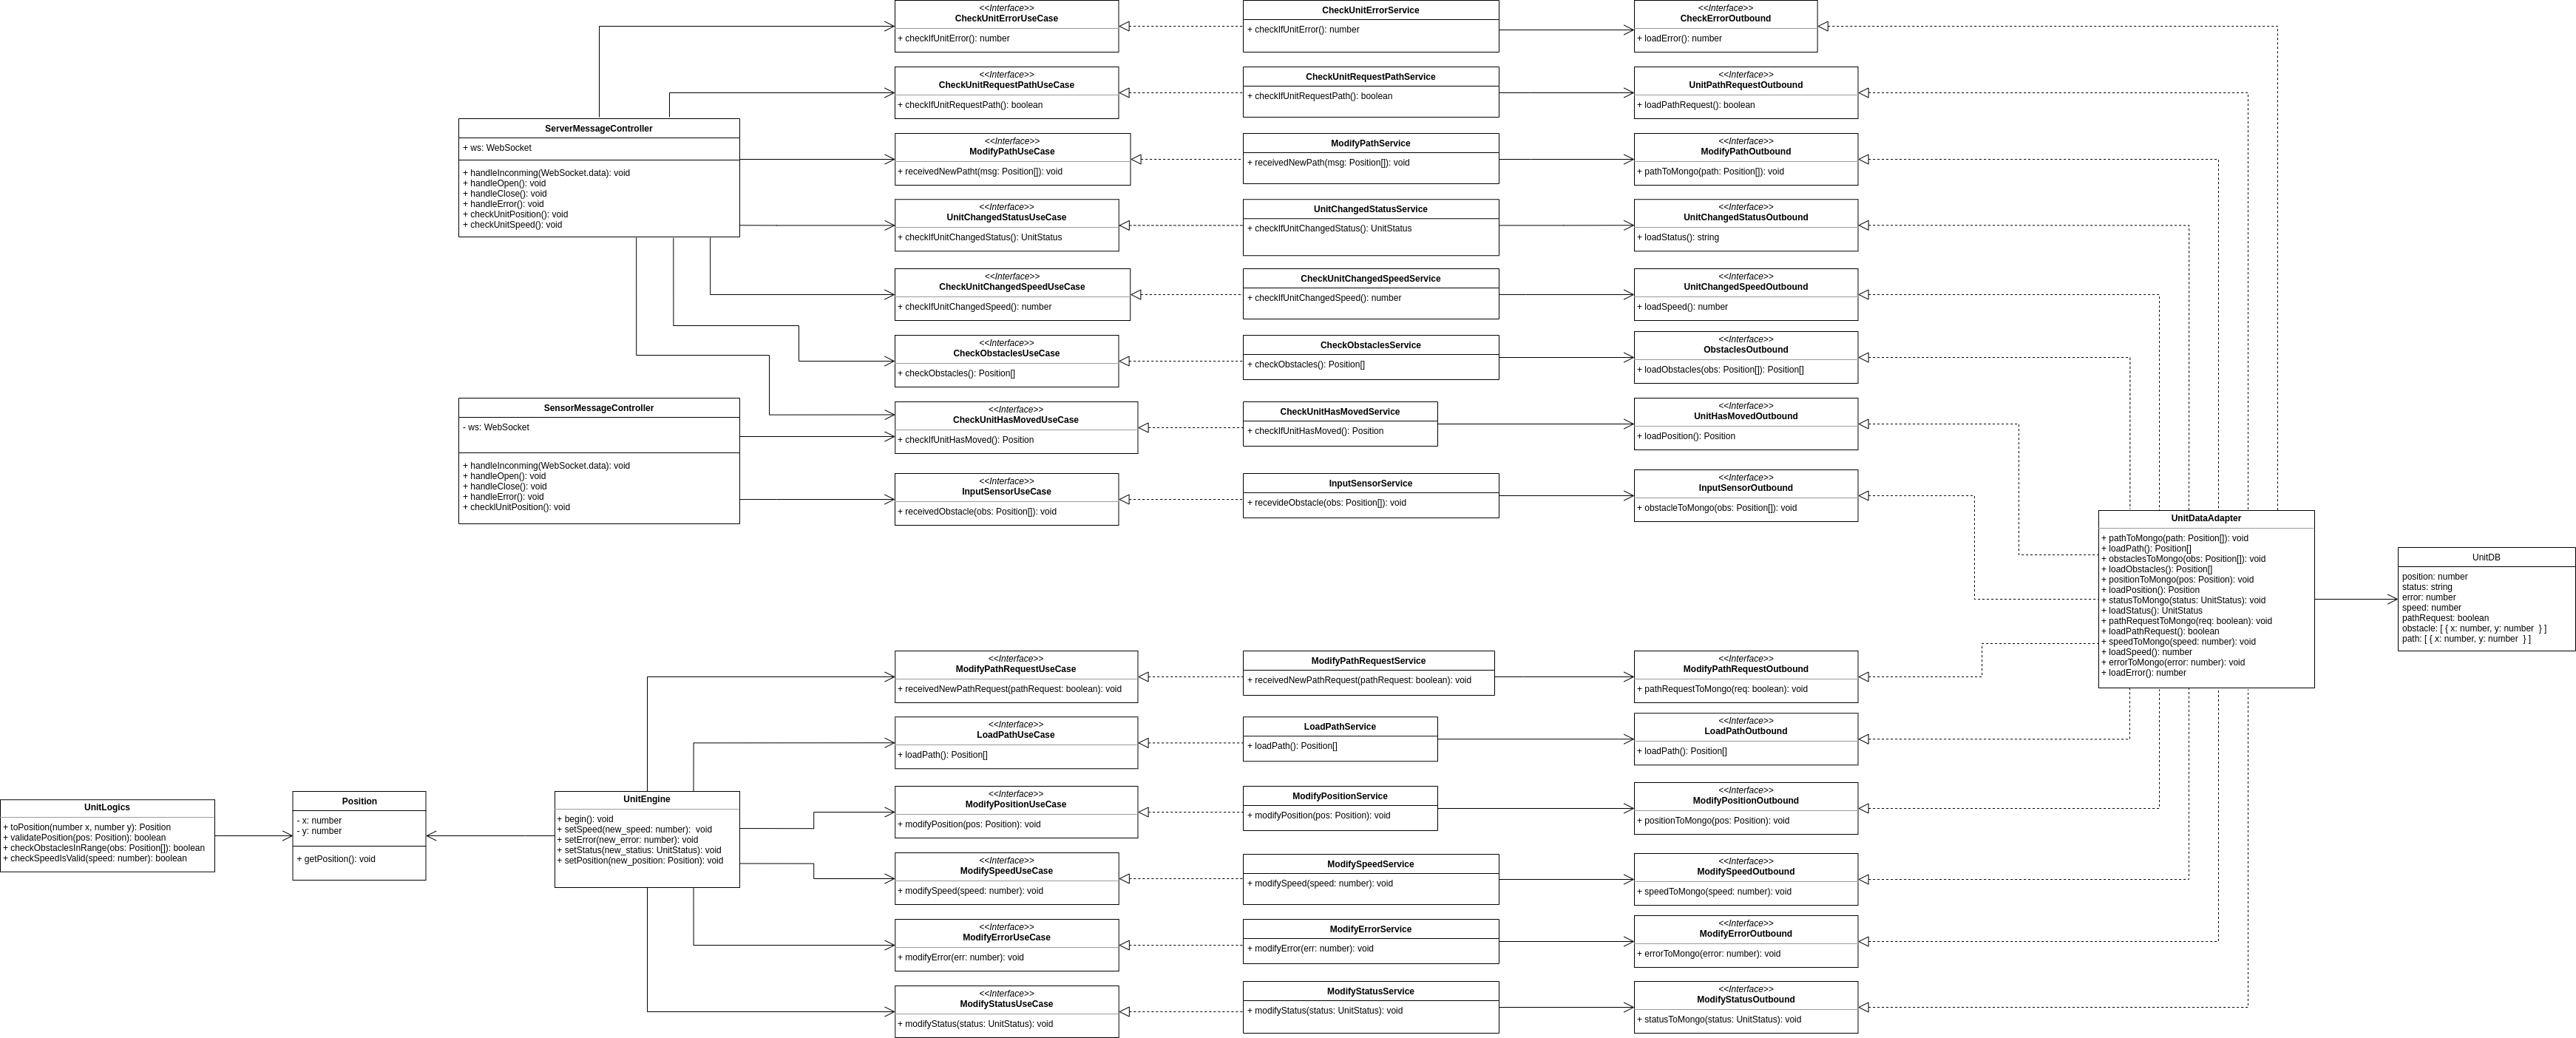
\includegraphics[width=25.5cm]{img/unit_architettura2.png}
			\caption{Unità - Diagramma delle classi}
		\end{figure}
	\end{landscape}
	
	
	\begin{landscape}
		\begin{figure}[H]
			\centering
			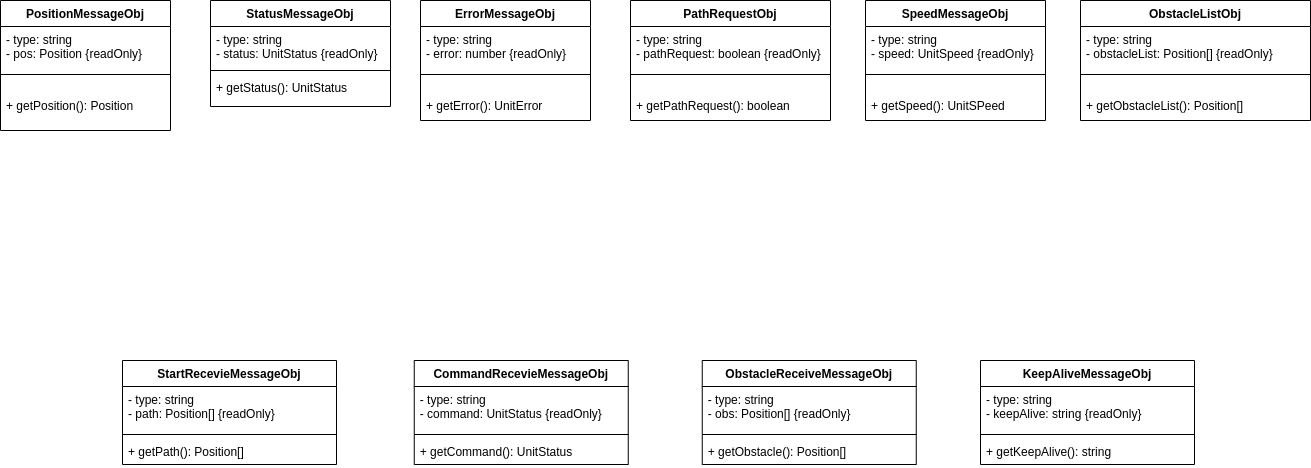
\includegraphics[width=25.5cm]{img/unit_messaggi.png}
			\caption{Unità - Messaggi}
		\end{figure}
	\end{landscape}
	\newpage

	\section{Manutenzione}
	\subsection{Aggiunta librerie}

\subsection{Aggiornamento librerie}

\subsection{Struttura progetto}

\subsection{Manutenzione dei test}

	\newpage

	\section{Espansione}
	\subsection{Server}
	La Layered Architecture prevede la netta separazione tra strati che facilita la sostituzione di un layer per intero oppure l'aggiunta di nuove funzionalità grazie alla creazione di nuove interfacce in uno specifico layer.
	\subsubsection{Supporto ad un nuovo database}
	Si potrebbe voler sostituire completamente il Persistence layer per passare da quello attuale con supporto a \glock{Redis} verso uno nuovo con supporto a database relazionale \glock{MariaDB}. L'interfaccia con il Business layer rimarrebbe immutata mentre cambierebbero solo le classi concrete incaricate di comunicare con il database.
	\subsubsection{Supporto ad un nuovo messaggio nell'API}
	Per aggiungere supporto a nuovi messaggi si dovrà lavorare sull'API layer aggiungendo una classe concreta che estenda la classe Message. A questo punto:
	\begin{itemize}
		\item se il messaggio è in uscita dal server si dovrà creare un Encoder che implementi l'interfaccia \textit{Encoder.Text<nome\_messaggio>};
		\item se invece è in ingresso allora bisognerà implementare il supporto a quel messaggio nei metodi \textit{decode} e \textit{willDecode} del Decoder specifico per l'Endpoint che riceverà il messaggio (UiMessageDecoder o UnitMessageDecoder).
	\end{itemize}

\subsection{UI}
	La UI si basa su Angular e supporta l'aggiunta di nuovi component come previsto dal framework. L'architettura della UI è Model-View-ViewModel e l'isolamento del Model rispetto ai ViewModel è garantito dall'interfaccia ServerService che viene implementata dal Model concreto. In caso di cambiamenti nell'API o nel protocollo di comunicazione il Model concreto può venire esteso o sostituito per intero mantenendo l'interfaccia ServerService invariata.
	
\subsection{Unità}
	L'unità è stata progettata secondo l'Hexagonal Architecture quindi ogni cambiamento nella relazione con componenti esterne (MongoDB, WebSocket) è dato dalla modifica o sostituzione degli Inbound Adapter e Outbound Adapter mantenendo invariate le Inbound Port e le Outbound Port.
	\newpage

	\section{Rilascio}
	La repository Git PORTACS contiene le repo delle tre componenti fondamentali (Server, UI e unità) come submodule e due script Bash, chiamati \textit{prepare} e \textit{reset}, per la preparazione delle immagini Docker.

\subsection{Preparazione}
Lo script \textit{prepare}, una volta lanciato, crea gli artefatti nei submodule e sulla base di questi inizializza le relative immagini Docker.
\\A questo punto il sistema di esecuzione dello script contiene le immagini Docker delle tre componenti che possono essere rilasciate su una repository Docker remota e successivamente caricate in produzione.

\subsection{Esecuzione}
L'immagine del server espone la porta TCP:8080 per la comunicazione tramite WebSocket con le unità e le UI, mentre l'immagine della UI espone la porta TCP:8081 per la comunicazione HTTP con il browser web al fine di visualizzare l'interfaccia grafica.

\subsection{Reset}
Lo script \textit{reset} cancella gli artefatti nei submodule e le immagini Docker create.
	\newpage

	\appendix
	\section{Glossario}
		\paragraph*{Angular}
	Framework open source per lo sviluppo di applicazioni web con licenza MIT, evoluzione di AngularJS.
	
	\paragraph*{AsciiDoc}
	Formato per documenti di testo che usa convenzioni di testo semplice come marcatori.
	
	\paragraph*{BIOS}
	Il Basic Input-Output System è il primo programma che viene eseguito dopo l'accensione, coinvolto pertanto nella fase di avvio (boot) del sistema di elaborazione.
	
	\paragraph*{Chai}
	Libreria di testing per Node.js e browser.
	
	\paragraph*{Checkstyle}
	Strumento di sviluppo per automatizzare il processo di controllo del codice Java. Aiuta a scrivere codice conforme a delle code conventions ben definite.
	
	\paragraph*{Continuous Integration}
	Pratica che si applica in contesti in cui lo sviluppo del software avviene attraverso un sistema di controllo versione. Consiste nell'allineamento frequente dagli ambienti di lavoro degli sviluppatori verso l'ambiente condiviso.
	
	\paragraph*{CSS}
	Cascaded Style Sheet, è un linguaggio che permette di definire tutte le proprietà di stile e formattazione di una pagina web in maniera modulare, tenendo questa parte della progettazione di un sito separata da quella relativa al contenuto.
	
	\paragraph*{Docker}
	Progetto open-source che automatizza la distribuzione di applicazioni all'interno di contenitori software, fornendo un'astrazione aggiuntiva grazie alla virtualizzazione a livello di sistema operativo di Linux.
	
	\paragraph*{ESLint}
	Strumento di analisi del codice statico per identificare i modelli problematici trovati nel codice JavaScript.
	
	\paragraph*{Framework}
	Architettura logica di supporto (spesso un'implementazione logica di un particolare design pattern) su cui un software può essere progettato e realizzato, spesso facilitandone lo sviluppo da parte del programmatore.
	
	\paragraph*{Git}
	Software di controllo versione distribuito utilizzabile da interfaccia a riga di comando.
	
	\paragraph*{GitHub}
	Servizio web di hosting per lo sviluppo di progetti software che usa il sistema di controllo di versione Git.
	
	\paragraph*{HTML}
	Linguaggio di markup per la strutturazione delle pagine web.
	
	\paragraph*{HTTP}
	Hypertext Transfer Protocol, è un protocollo a livello applicativo usato come principale sistema per la trasmissione d'informazioni sul web ovvero in un'architettura tipica client-server.
	
	\paragraph*{IDE}
	Integrated Development Environment, è un ambiente di sviluppo ovvero un software che, in fase di programmazione, supporta i programmatori nello sviluppo e debugging del codice sorgente di un programma.
	
	\paragraph*{IntelliJ IDEA}
	Ambiente di sviluppo integrato per il linguaggio di programmazione Java.
	
	\paragraph*{Jackson}
	Libreria ad alte prestazioni per Java che processa istanze trasformandole in JSON e viceversa.
	
	\paragraph*{Jasmine}
	Framework di test open source per JavaScript.
	
	\paragraph*{Java}
	Linguaggio di programmazione ad alto livello, orientato agli oggetti e a tipizzazione statica, che si appoggia sull'omonima piattaforma software di esecuzione, specificamente progettato per essere il più possibile indipendente dalla piattaforma hardware di esecuzione tramite l'utilizzo di macchina virtuale.
	
	\paragraph*{Javascript}
	Linguaggio di scripting orientato agli oggetti e agli eventi, utilizzato nella programmazione Web sia lato client che server.
	
	\paragraph*{JSON}
	Acronimo di JavaScript Object Notation, è un formato di file adatto all'interscambio di dati fra applicazioni client/server.
	
	\paragraph*{JUnit}
	Framework di unit testing per il linguaggio di programmazione Java.
	
	\paragraph*{LaTeX}
	Linguaggio di markup per la preparazione di testi, basato sul programma di composizione tipografica TEX.
	
	\paragraph*{MariaDB}
	MariaDB è un DBMS nato da un fork di MySQL creato dal programmatore originale di tale programma.
	
	\paragraph*{Maven}
	Strumento completo per la gestione di progetti software Java, in termini di compilazione del codice, distribuzione, documentazione e collaborazione del team di sviluppo.
	
	\paragraph*{Mocha}
	Framework di test JavaScript per i programmi Node.js, con supporto per browser, test asincroni, rapporti sulla copertura dei test e utilizzo di qualsiasi libreria di asserzioni.
	
	\paragraph*{MongoDB}
	DBMS non relazionale, orientato ai documenti.
	
	\paragraph*{Node.js}
	Runtime di JavaScript Open source multipiattaforma orientato agli eventi per l'esecuzione di codice JavaScript.
	
	\paragraph*{NPM}
	Node Package Manager, è un gestore di pacchetti per il linguaggio di programmazione JavaScript. È il gestore di pacchetti predefinito per l'ambiente di runtime JavaScript Node.js. Consiste in un client da linea di comando, chiamato anch'esso npm e un database online di pacchetti pubblici e privati, chiamato npm registry.
	
	\paragraph*{POI}
	Point Of Interest, è un punto specifico che qualcuno potrebbe trovare utile o interessante.
	
	\paragraph*{Redis}
	Database chiave-valore open-source residente in memoria con persistenza facoltativa.
	
	\paragraph*{SonarCloud}
	Servizio Cloud per la misurazione della qualità di un prodotto software tramite analisi statica del codice.

	\paragraph*{Typescript}
	Linguaggio di programmazione open-source sviluppato da Microsoft che estende il linguaggio Javascript aggiungendo alcuni costrutti sintattici.
	
	\paragraph*{WebSocket}
	È una tecnologia web che fornisce canali di comunicazione full-duplex attraverso una singola connessione TCP.
	\newpage

\end{document}